\documentclass[tikz,border=10pt]{standalone}
\usetikzlibrary{matrix, positioning, arrows.meta}

\begin{document}
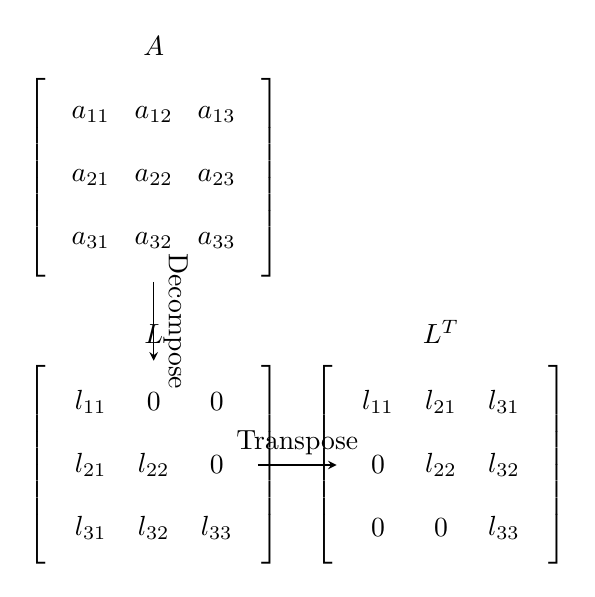
\begin{tikzpicture}[
    matrixstyle/.style={
        matrix of math nodes,
        left delimiter={[},
        right delimiter={]},
        nodes={minimum width=8mm, minimum height=8mm, anchor=center},
    },
    arrowstyle/.style={->,>=stealth}
]

% Matrix A
\matrix (A) [matrixstyle] {
    a_{11} & a_{12} & a_{13} \\
    a_{21} & a_{22} & a_{23} \\
    a_{31} & a_{32} & a_{33} \\
};
\node[above=1mm of A] (labelA) {$A$};

% Matrix L
\matrix (L) [matrixstyle, below=of A.south west, anchor=north west] {
    l_{11} & 0 & 0 \\
    l_{21} & l_{22} & 0 \\
    l_{31} & l_{32} & l_{33} \\
};
\node[above=1mm of L] (labelL) {$L$};

% Matrix L Transpose
\matrix (LT) [matrixstyle, right=of L] {
    l_{11} & l_{21} & l_{31} \\
    0 & l_{22} & l_{32} \\
    0 & 0 & l_{33} \\
};
\node[above=1mm of LT] (labelLT) {$L^T$};

% Arrows
\draw[arrowstyle] (A) -- (L) node[midway, above, sloped] {Decompose};
\draw[arrowstyle] (L) -- (LT) node[midway, above] {Transpose};

\end{tikzpicture}
\end{document}
